\chapter{Защита от подделывания радужки}
\label{chapter:anti-spoofing}

Способность обеспечивать надежную защиту от попыток подделывания является одним из ключевых требований к системе безопасности, использующей биометрические методы. Распознавание по радужной оболочке глаза является одной из наиболее перспективных и новых биометрических технологий на рынке мобильных устройств (\ref{sec:beometric_methods_applications},~\ref{sec:mobile_iris_features}). О преимуществах технологии по сравнению с иными биометрическими методами упоминалось ранее (\ref{sec:beometric_methods_overview}). За последние годы несколько компаний представили технологию аутентификации по радужке, встроенную в свои смартфоны, среди наиболее известных:~\cite{deltaId,lumia_950,samsung_iris}. Предполагается, методы биометрической аутентификации станут заменой для привычных схем с паролями. В целом технология предназначена для более удобного взаимодействия с устройством и, в то же время, для повышения уровня безопасности личной информации пользователя, хранящейся на устройстве.

После выпуска устройств, оснащенных сканером радужки, стали подтверждаться факты взлома технологии путем подделывания (спуфинга, spoofing) радужной оболочки глаза и представлении её устройству в качестве оригинальной, принадлежащей пользователю. Следует отметить, что попытки взлома предпринимались группами профессионалов, специализирующимися на взломе и компрометировании технологий безопасности, в т.ч. и биометрических ~\cite{ccc,bkav}. Эксперименты проведенные в рамках данного настоящего исследования подтверждают, что идеи обоих упомянутых методов спуфинга являются выполнимыми, за исключением нескольких важных условий, которые должны быть выполнены: изображение радужной оболочки должно быть захвачено инфракрасной камерой с высоким разрешением таким образом, что диаметр радужки на изображении должен составлять не менее 250-300 точек на бумаге, напечатанной с разрешением не менее 600 dpi, что означает, что изображение должно быть зафиксировано либо с очень короткого расстояния, либо с использованием телеобъектива с высоким разрешением; глаза должны быть открыты достаточно с прицелом, направленным к камере; изображение радужной оболочки не должно быть размытым и недооцененным; Таким образом, можно сделать вывод, что проблема анти-спуфинга радужки остается актуальной, в особенности для мобильных приложений.

\section{Обзор методов защиты от подделывания радужки}
\label{sec:anti-spoofing-methods-overview}

Среди известных способов спуфинга радужки можно выделить следующие~\cite{he_2009_s,galbally_2012,czajka_2018}: представление системе напечатанной на принтере с высоким разрешением изображении радужки пользователя; представление изображения либо последовательности изображений радужки с экрана другого устройства; представление системе искусственного глаза, изготовленного из стекла или пластика; представление контактной линзы с рисунком оригинальной радужки пользователя; иные возможные варианты, позволяющие обеспечить реалистичность радужки для биометрической системы.

Cуществующие методы борьбы с подделыванием радужки, описанные в литературе, могут быть поделены на:

\begin{enumerate}
	\item[$\bullet$] Использующие и не использующие дополнительные аппаратные средства, позволяющие обнаруживать особые физиологические свойства <<живности>> радужки, например глазного гиппуса, представляющего собой естественное колебание диаметра зрачка в ответ на внезапное изменение освещения (например, включение дополнительного диода)~\cite{galbally_2012,czajka_2018};
	\item[$\bullet$] Требующие и не требующие дополнительного взаимодействия с пользователем, например посредством вывода подсказок с просьбой закрыть/открыть веки, предоставить иную дополнительную информацию в виде пин-кода и др.
\end{enumerate}

Класс методов, использующих дополнительные аппаратные средства, а также требующие дополнительного взаимодействия с пользователем, рассматривается в меньшей степени, когда речь заходит о их применении на мобильном устройстве, главным образом потому, что такой подход может значительно увеличить стоимость и, в то же время, уменьшить удобство использования технологии~\cite{odinokikh_antispoofing_2018}. Полностью автоматические подходы выделяются экономичностью, что делает их привлекательными для коммерческого применения, однако, требуют высокой степени универсальности и устойчивости к изменениям выходных данных.

Одной из первых работ в данной области была~\cite{daugman_antispoofing_2004}, в которой рассматривалась проблема спуфинга при помощи напечатанных на бумаге изображения радужки. В работе утверждалось, что процесс печати оставляет обнаруживаемые следы на поддельных образцах и предлагалось их обнаружение применением двумерного анализа Фурье полученного изображения. Подход показал свою эффективность против атак с использованием изображений радужки, напечатанных на бумаге. Однако, метод оказался неустойчивым к иным видам атак, описанными далее. Несколько методов анализа признаков, присущих искусственным радужкам в частотной области, были предложены в работах~\cite{he_2008} и ~\cite{czajka_2013}. В работе ~\cite{raja_2015} предлагается метод представления изображения радужки в виде пирамиды Лапласа для различных масштабов. Метод позволяет анализировать частотные отклики для разных ориентаций радужки и обнаруживать артефакты, присущие искусственным образцам, с использованием последовательности изображений. Методы, основанные на локальных дескрипторах, также используются для анализа и представления текстуры радужки с целью обнаружения спуфинг-атак. Например, в работах ~\cite{he_2008,gupta_2014} показана эффективность использования различных конфигураций LBP (local binary patterns, локальных бинарных шаблонов) дескрипторов против ряда известных атак (например, контактные линзы с рисунком радужки, напечатанные на бумаге, искусственные радужки из пластика или стекла т. д.). Бинарные особенности изображения, основанные на статистиках (BSIF) также изучались в контексте обнаружения подделок и тестировались на разных базах данных подделок~\cite{raghavendra_2015}. Комплексное решение для защиты от спуфинга на основе комбинации нескольких локальных дескрипторов (LBP, BSIF и локального квантования фазы (LPQ)) для представления текстуры представлено в комплексном исследовании ~\cite{gragnaniello_2015}.

В работе~\cite{galbally_2012} было показано, что различные метрики качества изображения радужки могут быть использованы для обнаружение спуфинг-атак. Идея подхода исходит из предположения о том, что входные изображения подделок могут значительно отличаться по уровню качества от оригинальных для нормальных (фиксированных) условий распознавания. Несколько значимых в отношении детектирования подделок метрик качества представлены в работе~\cite{galbally_2012} и протестированы на образцах подделок, напечатанных на бумаге.

Одним из наиболее многообещающих подходов к детектированию спуфинг-атак сегодня является применение методов глубокого обучения. Такие методы демонстрируют высокую надежность по сравнению с существующими. Одной из пионерских работ в применении к радужке, лицу и отпечаткам пальцев была~\cite{menotti_2015}. Комплексная работа по сравнении различных подходах регулярно организовывается в рамках LivDet соревнований, где методы глубокого обучения по результатам последних лет занимают лидирующие позиции~\cite{livdet_2013,livdet_2015,livdet_2017}.

Все вышеупомянутые подходы к обнаружению спуфинг-атак были рассмотрены в контексте мобильных приложений, накладывающих на них дополнительные ограничения, о которых говорилось ранее (\ref{sec:main_difficulties_mobile}, \ref{sec:mobile_iris_features}). Среди всех, для сравнения были выбраны~\cite{sequeira_2014,sequeira_2014_2,raghavendra_2015}, которые отвечали требованиям мобильных приложений, демонстрирующие при этом перспективные результаты.

\section{Обнаружение подделок радужки методами глубокого обучения}
\label{sec:proposed-anti-spoofing}

Предложен универсальный метод обнаружения спуфинг-атак разных категорий. Метод основан на использовании моделей глубоких сверточных нейронных сетей (CNN). Входными данными метода являются два изображения: изображение радужки $I_{ER}$, центр которого совпадает с центром радужки, и изображение нормализованной радужки $I_{NI}$, получаемое преобразованием вида \ref{eq:certesian-polar},~\ref{eq:certesian-polar2}. Примеры обоих изображений приведены на Рис.~\ref{fig:anti-spoofing-arch-scheme}. Метод опирается на информацию о положении и размерах зрачка и радужки, которые, в простейшем случае, могут быть описаны параметрически окружностями.

\begin{figure}[t!]
	\centering
	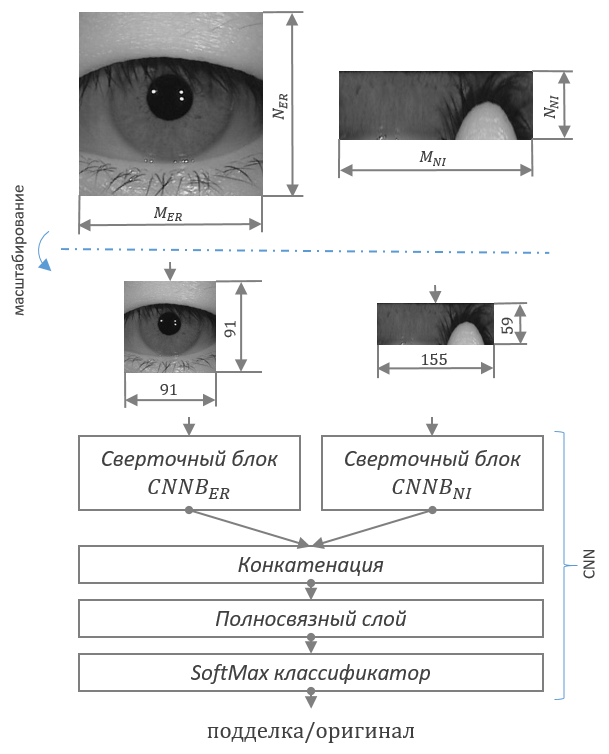
\includegraphics[width=0.75\columnwidth]{pictures/anti-spoofing-arch-scheme.png}
	\caption{Общая схема алгоритма защиты от подделывания радужки}
	\label{fig:anti-spoofing-arch-scheme}
\end{figure}

Проверка на наличие потенциальной спуф-атаки производится сразу после этапа нормализации радужки (описан в разделе~\ref{sec:iris_recognition_basics}) и состоит из двух этапов: масштабирование изображения и пропускания его через сверточную нейронную сеть (Рис.~\ref{fig:anti-spoofing-arch-scheme}). Изображение области радужки $I_{ER}(M_{ER},N_{ER})$ вырезается с пропорцией $M_{ER}=N_{ER}=3R_i$, где $R_i$ - радиус радужки. Центр изображения $I_{ER}$ совмещен с центром радужки, описываемой окружностью.

Далее обе изображения масштабируются до заранее заданного размера в пикселях (Рис.~\ref{fig:anti-spoofing-arch-scheme}). Размер изображения выбирается заранее как оптимальный для заданной архитектуры и позволяющий обеспечивать достаточную точность и скорость обработки для полученной модели.

{\bf Архитектура сверточной сети}
\label{sec:proposed-anti-spoofing-architecture}

Предложенный метод основан на использовании основных блоков архитектуры MobileNet~\cite{howard_2017}, показавшей свою эффективность и применимость для задач, связанных с мобильными приложениями. Одно из основных преимуществ архитектуры это конструкция её основных сверточных блоков. Пары слоев сверток по глубине (depth-wise convolutions) с последующими свертками с ядрами 1х1 позволяют существенно снизить количество умножений, сохраняя емкостные характеристики модели~\cite{howard_2017}.

Пары изображений $I_{ER}$ и $I_{NI}$, полученные из одного исходного изображения подаются на вход сверточным блокам $CNNB_{ER}$ и $CNNB_{NI}$ соответственно, как показано на Рис.~\ref{fig:anti-spoofing-arch-scheme}. Структура обоих блоков отражена в Таб.~\ref{tab:erniblock}. Блоки имеют схожую структуру, основными элементами которой являются структурные единицы архитектуры MobileNet~\cite{howard_2017}, обозначенные как $CNNB_{MN}$. Структура блоков $CNNB_{MN}$ описана в Таб.~\ref{tab:dwscblock}.

\begin{table}[h]
	\begin{center}
		\begin{tabular}{|c|c|c|c|}
			\hline
			\textbf{Элемент архитектуры}								& \multicolumn{2}{|c|}{\textbf{Размер входного тензора}} \\
			\cline{2-3}
			\textbf{блока}												& $CNNB_{ER}$				& $CNNB_{NI}$ \\
			\hline
			Сверточный слой $(k_h=k_w=3,s'=2)$							& $1\times91\times91$		& $1\times59\times123$\\
			Сверточный блок $CNNB_{MN} (k_h=k_w=3,s'=1)$ 				& $8\times45\times45$		& $8\times29\times61$\\
			Сверточный блок $CNNB_{MN} (k_h=k_w=3,s'=2)$ 				& $16\times43\times43$		& $16\times27\times59$\\
			Сверточный блок $CNNB_{MN} (k_h=k_w=3,s'=1)$ 				& $32\times21\times21$		& $32\times13\times29$\\
			Сверточный блок $CNNB_{MN} (k_h=k_w=3,s'=2)$ 				& $64\times19\times19$		& $64\times11\times29$\\
			Сверточный блок $CNNB_{MN} (k_h=k_w=3,s'=1)$ 				& $64\times9\times9$		& $64\times5\times13$\\
			Глобальный усредняющий пуллинг								& $64\times7\times7$		& $64\times3\times11$\\
			\hline
		\end{tabular}
	\caption{Структура блоков $CNNB_{ER}$ и $CNNB_{NI}$: $k_h,k_w$ - размеры ядра свертки по вертикали и горизонтали соответственно}
	\label{tab:erniblock}
	\end{center}
\end{table}

Над картами признаков, полученных для изображений $I_{ER}$ и $I_{NI}$ на выходе из соответствующих блоков, производится операция глобального усредняющего пулинга (global average pooling). Затем они объединяются в один вектор, являющийся входом последнего полносвязного (fully-connected) слоя. Классификатор softmax используется для оценивания вероятностей $P_{spoof}$ and $P_{live}$ принадлежности текущего изображения к одному из двух классов: живой или подделка.

Предложенная модификация архитектуры имеет намного меньшее количество параметров по сравнению с оригинальной~\cite{howard_2017}, а также использует отступы (paddings) типа <<valid>>, что позволяет уменьшить количество операций при прямом проходе (forward pass).

{\bf Описание базы данных подделок}
\label{sec:spoof-dataset-description}

На сегодняшний день доступно несколько баз данных, содержащих изображения оригинальных (живых) радужек и подделок.
По аналогии с наборами данных, собранными для оценки эффективности распознавания радужки, их можно разделить на две группы: полученные в видимом и ближнем инфракрасном (БИК) спектрах. Поскольку системы, использующие БИК изображения, более распространены в виду ряда преимуществ, упомянутых ранее (\ref{sec:iris_recognition_basics},~\ref{sec:auth_method}), в работе рассмотрены только изображения, полученные в БИК диапазоне. В смежных работах также рассмотрено несколько распространенных типов подделок, среди которых: радужка, напечатанная на бумаге; живая радужка, покрытая текстурированными (узорчатыми) контактными линзами; живая радужка, покрытая полу-прозрачной контактной линзой, с воспроизведенным на ней рисунком радужки какого-либо человека. Случай с воспроизведением рисунка радужки пользователя устройства кажется слишком сложным в реализации, поэтому не рассматривается в данной работе. Сценарий атаки с радужкой, напечатанной на бумаге, более прост и интуитивен. В некторых из самых недавних работ в области сообщается, что такую проблему удалось решить, однако, ни в одной из них не рассматривается использование технологии в мобильном устройстве.

На сегодняшний день не существует доступных наборов данных, полученных при помощи мобильного устройства в БИК диапазоне. По этой причине такой набор данных был предварительно собран. Набор включает в себя следующие типа атак, часть из которых не была рассмотрена ранее: (i) изображение радужки, напечатанное на бумаге (PR); (ii) изображение радужки, напечатанное на бумаге с наложением прозрачных контактных линз (PWL); (iii) изображение радужки, напечатанное на бумаге с нанесением прозрачного клея (PWG). Такие типы образцов подделок были выбраны не случайно. Именно они были успешно использованы для обхода мобильной биометрической системы ~\cite{ccc,bkav}. Изображения радужной оболочки были получены с использованием NIR-камеры высокого разрешения в диапазоне расстояний от 20 до 40 (см) и далее напечатаны на белой бумаге с разрешениями 600/1200 (dpi) в равной пропорции. Полученные образцы были использованы для съемки примеров трех классов подделок. В качестве примеров живых радужек были выбраны две категории: (i) изображение радужки, полученно при нормальном освещении внутри хорошо освещенной комнаты (IN); (ii) изображение радужки, полученные в солнечную погоду вне помещения (OUT). Данные категории были выбраны из соображений рассмотрения возможности изменения условий окружения, присущих мобильным приложениям.

В качестве устройства для регистрации изображения было выбрано портативное вычислительное устройство Raspberry Pi с камерой (PiCamera v2.1) с дополнительно установленным полосно-пропускающим ($850\pm20$ нм) БИК фильтром, позволяющей получать изображения в БИК диапазоне частот. В качестве дополнительного источника освещения был использован светодиод с пиковой частотой излучения 850 нм. детальная информация о собранном наборе данных представлена в Таб.~\ref{tab:spoof-dbdescription}. Разбиение данных на обучающую и тестовую выборку производилось таким образом, чтобы наборы не пересекались по субъектам. Несколько примеров изображений $I_{ER}$ из набора представлены на Рис.~\ref{fig:spoof-samples}.

\begin{table}[t]
	\caption{Описание собранно базы данных (живой/подделка) радужек}
	\begin{center}
		\begin{tabular}{|c|c|}
			\hline
			\textbf{Параметр}							&\textbf{Значение} \\
			\hline
			Разрешение изображения 						&	$320\times240$\\
			Кол-во субъектов/глаз						&	$23/46$\\
			Кол-во изображений подделка/живой			&	$18548/18031$\\
			IN/OUT/PR/PWL/PWG (весь набор)				& 	$10679/7869/6233/5907/5891$\\
			IN/OUT/PR/PWL/PWG (тестовый набор)			& 	$2534/2006/1436/1452/1568$\\
			\hline
		\end{tabular}
		\label{tab:spoof-dbdescription}
	\end{center}
\end{table}

\begin{figure}[t!]
	\centering
	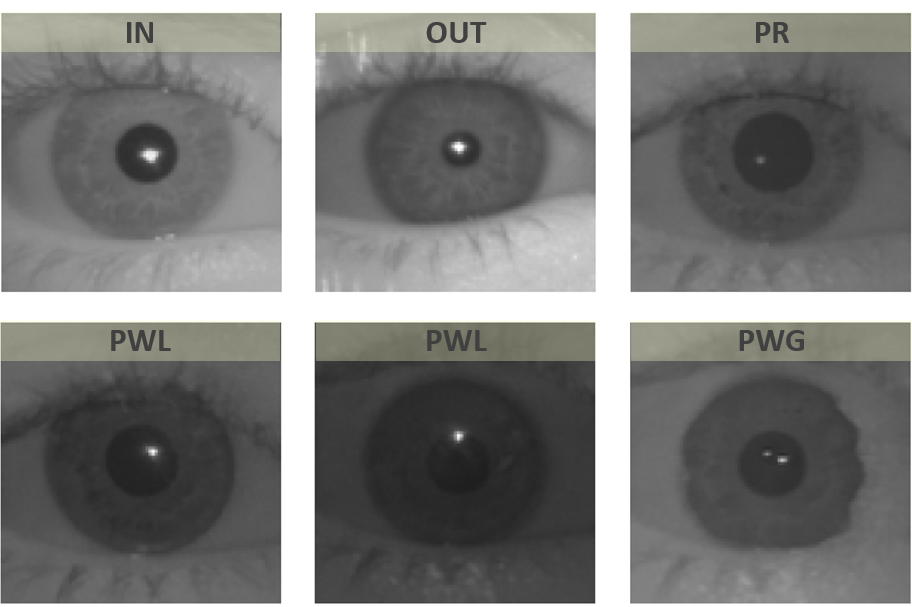
\includegraphics[width=0.75\columnwidth]{pictures/spoof-samples.png}
	\caption{Примеры изображений}
	\label{fig:spoof-samples}
\end{figure}

{\bf Экспермиентальные результаты}
\label{sec:anti-spoofing-experimental}

Для того чтобы оценить эффективность предлагаемого решения, были реализованы несколько известных литературы методов. Производительность методов оценивалась на собранном, упомянутом выше наборе данных. Среди известных подходов: методы, в основе которых лежит частотный анализ, предложенные в работах~\cite{czajka_2013} и~\cite{he_2008}; метод, построенный на LBP~\cite{gupta_2014} и BSIF дескрипторах~\cite{raghavendra_2015}, а также метод, предложенный в работе~\cite{sequeira_2014_2} с использованием численных показателей качества изображения. Вышеупомянутые методы были выбраны как демонстрирующие наивысшую производительность на наборах данных изображений, полученных в БИК диапазоне согласно обзору, приведенному в работе~\cite{galbally_2016}. По причине высокой вычислительной сложности метод, основанный на применении пары CNN в сочетании с набором решающих правил, предложенных исследователями из CASIA в работе~\cite{livdet_2017}, был исключен из рассмотрения как неприменимый для мобильных приложений, работающих в режиме реального времени. Время выполнения для метода в 400 раз превышает время для метода, предложенного в данной работе.

Для оценивания точности распознавания были выбраны следующие показатели: \textit{FerrLive} - доля изображений живых образцов, ошибочно классифицированных как подделки; \textit{FerrFake} - доля изображений подделок, ошибочно классифицированных как живые; \textit{CCR (correct classification rate)} - доля правильно классифицированных изображений на всем наборе данных. В Таб.~\ref{tab:anti-spoofing-expresults} приведены результаты тестирования известных из литературы и предложенного методов. Важно отметить, что только два из упомянутых решений (\cite{raghavendra_2015} и~\cite{sequeira_2014_2}) были изначально представлены как способные обеспечивать возможность использования в мобильном устройстве. К преимуществам метода~\cite{sequeira_2014_2} можно отвести простоту и относительное быстродействие алгоритма. Метод, предложенный в работе~\cite{raghavendra_2015} включает в себя вычислительно сложные операции свертки с фильтрами относительно большой размерности: от $7\times7$ до $17\times17$, что делает его менее предпочтительным для развертывания на мобильном устройстве.

\begin{table}[t]
	\caption{Результаты по точности классификации живых радужек и подделок}
	\begin{center}
		\begin{tabular}{|c|c|c|c|c|c|c|c|c|}
			\hline
			\textbf{Method}								& \textbf{FerrLive} & \textbf{FerrFake} & \textbf{CCR}      \\
			\hline
			Czajka~\cite{czajka_2013}					& $0.505$          & $0.207$          & $0.661$          \\
			He~\cite{he_2008}							& $0.370$          & $0.739$          & $0.442$          \\
			Gupta~\cite{gupta_2014}						& $0.294$          & $0.251$          & $0.749$          \\
			Raghavendra~\cite{raghavendra_2015}			& $0.076$           & $0.128$          & $0.897$          \\
			Sequeira~\cite{sequeira_2014_2}				& $0.320$          & $0.293$          & $0.694$          \\
			\textbf{Предложенный метод}					& $\mathbf{0.048}$  & $\mathbf{0.034}$  & $\mathbf{0.959}$ \\
			\hline
		\end{tabular}
		\label{tab:anti-spoofing-expresults}
	\end{center}
\end{table}

Тестирование предложенного метода производилось на мобильном устройстве. Полное медианное время выполнения измерено на процессоре Qualcomm Snapdragon 835 CPU (2.45 GHz) и составило 4-6 миллисекунд. Измерения производились на одном ядре процессора.

\section{Выводы к пятой главе}
\label{sec:conclusion-5}

Рассмотрены особенности защиты от подделывания радужек в применении к распознаванию с мобильного устройства. Воспроизведены попытки взлома при помощи методов, использованных группами профессиональных взломщиков. Произведена классификация общих подходов к защите от подделывания. Произведен обзор существующих методов, рассмотрены их преимущества и недостатки. Рассмотрены новые виды подделок, ранее не исследовавшиеся в литературе: (i) изображение радужки, напечатанное на бумаге с наложением прозрачных контактных линз; (ii) изображение радужки, напечатанное на бумаге с нанесением прозрачного клея. Собрана и обработана база данных изображений в том числе новых видом подделок при помощи мобильного устройства с учетом возможных изменений окружения. Разработан, протестирован и внедрен новый метод защиты от спуфинг-атак, основанный на применении методов глубокого обучения, в частности, сверточных нейронный сетей. Предложенный метод продемонстрировал высокую точность обнаружения подделок, значительно превосходящую известные из литературы решения, а также скорость обработки, достаточную для запуска на мобильном устройстве в режиме реального времени.
